
%%%%%%%%%%%%%%%%%%%%%%%%%%%%%%%%%%%%%%%%%%%%%%%%%%%%%%%%%%%%%%%%%%%%%%%%%%%%%
\chapt[chap:cloud]{GATE Cloud}
\markboth{GATE Cloud}{GATE Cloud}
%%%%%%%%%%%%%%%%%%%%%%%%%%%%%%%%%%%%%%%%%%%%%%%%%%%%%%%%%%%%%%%%%%%%%%%%%%%%%
\nnormalsize

%%%%%%%%%%%%%%%%%%%%%%%%%%%%%%%%%%%%%%%
%\sect[sec:family:cloud]{GATE Cloud}

The growth of unstructured content on the internet has resulted in an increased need 
for researchers in diverse fields to run language processing and text mining on 
large-scale datasets, many of which are impossible to process in reasonable time on 
standard desktops. However, in order to take advantage of the on-demand compute 
power and data storage on the cloud, NLP researchers currently have to re-write/adapt 
their algorithms. 

Therefore, we have now adapted the GATE infrastructure 
(and its JAPE rule-based and machine learning engines) to the cloud and thus enabled 
researchers to run their GATE applications without a significant overhead. 
In addition to lowering the barrier to entry, GATE Cloud also reduces the time 
required to carry out large-scale NLP experiments by allowing researchers to 
harness the on-demand compute power of the cloud. 

Cloud computing means many things in many contexts. On \htlink{http://cloud.gate.ac.uk}{GATE Cloud} it
means:

\begin{itemize}
\item {\bf zero fixed costs}: you don't buy software licences or server hardware, just
  pay for the compute time that you use.
\item {\bf near zero startup time}: in a matter of minutes you can specify, provision
  and deploy the type of computation that used to take months of planning.
\item {\bf easy in, easy out}: if you try it and don't like it, go elsewhere! You can
  even take the software with you; it's all open-source.
\item {\bf someone else takes the admin load}:
  - \htlink{http://gate.ac.uk/}{the GATE team} from the 
    \htlink{http://www.shef.ac.uk/}{University of Sheffield} make sure you're running the best of breed
    technology for text, search and semantics.
\item cloud providers' data center managers (we use 
    \htlink{http://aws.amazon.com/}{Amazon Inc.}) make sure the hardware and operating platform for your work
    is scaleable, reliable and cheap.
\end{itemize}

\htlink{http://gate.ac.uk}{GATE} is (and always will be) free, but machine time,
training, dedicated support and bespoke development is not. Using GATE Cloud
you can rent cloud time to process large batches of documents on vast server
farms, or academic clusters. You can push a terabyte of annotated data into an
index server and replicate the data across the world. Or just purchase
training services and support for the various tools in the
\htlink{http://gate.ac.uk/family/}{GATE family}.
%%%%%%%%%%%%%%%%%%%%%%%%%%%%%%%%%%%%%%%%%%%%%%%%%%%%%%%%%%%%%%%%%%%%%%
\sect[sec:family:cloud-services]{GATE Cloud services: an overview}
%%%%%%%%%%%%%%%%%%%%%%%%%%%%%%%%%%%%%%%%%%%%%%%%%%%%%%%%%%%%%%%%%%%%%%
%
GATE Cloud offers several types of services:
\begin{itemize}
\item Run a pre-packaged annotation pipeline such as ANNIE or TwitIE.
  Individual documents can be processed free of charge using a REST API (rate
  limits apply) or larger batches of documents can be processed using the paid
  service described below.
\item Uniquely among online text-mining platforms, the batch-mode service also
  allows you to build your own custom pipeline in GATE Developer and upload it
  to run on the cloud infrastructure.
\item Rent a dedicated server to index your documents using GATE M\'{i}mir
  (chapter~\ref{chap:mimir}), or to collect social media data via Twitter's
  streaming APIs.
\end{itemize}

For an up to date list of available services see
\htlinkplain{https://cloud.gate.ac.uk/shopfront}.


%%%%%%%%%%%%%%%%%%%%%%%%%%%%%%%%%%%%%%%%%%%%%%%%%
\sect[sec:family:cloud-buy]{Using GATE Cloud services}
%%%%%%%%%%%%%%%%%%%%%%%%%%%%%%%%%%%%%%%%%%%%%%%%%

The GATE Cloud platform is designed to make it easy for you to explore the
available resources and experiment with them to find one (or more) that suits
your needs. You can browse the available services and filter the pipelines and
dedicated servers by tag. You can "try before you buy" -- the detail page for
each pipeline has a simple tool to allow you to paste in or upload a small
sample of text, run the pipeline over the text, and browse the resulting
annotations.

Once you have found a pipeline of interest you can use the on-line REST API to
process documents free of charge.  The basic quota allows you to process 1,200
documents per day at an average rate of 2 per second, but higher quotas are
available for research users or by commercial arrangement with the GATE team.
To use the API, first sign up for an account on GATE Cloud, then visit your
account management page to generate an API key.  There are links to client
libraries and API documentation on the GATE Cloud site.

For other services -- batch processing with one of the standard pipelines or
one of your own, and dedicated Twitter collection or \Mimir\ servers -- you
will need to buy credit vouchers from the
\htlink{http://onlineshop.shef.ac.uk/browse/product.asp?compid=1\&modid=1\&catid=97}
{University of Sheffield online shop}.  Vouchers are available in any multiple
of \textsterling 5, and you can buy additional vouchers at any time.  Note that
you \emph{must} use exactly the same email address on the University shop as on
your GATE Cloud account, in order for us to be able to match up your purchases
and apply the credit to your account automatically.  With the batch mode service
there are \textbf{no limits} on the number or size of documents you can process,
you simply pay for the amount of processing time you use and the amount of data
you want to store, with a simple and transparent pricing structure.

As with the free quotas, we can offer discounts on the price of paid services
for research users -- contact us for more details.



%%%%%%%%%%%%%%%%%%%%%%%%%%%%%%%%%%%%%%%%%%%%%%%%%%%%%%%%%%%%%%%%%%%%%%%%%%%%%
\sect[sec:family:cloud-annotation-jobs]{Annotation Jobs on GATE Cloud}
%%%%%%%%%%%%%%%%%%%%%%%%%%%%%%%%%%%%%%%%%%%%%%%%%%%%%%%%%%%%%%%%%%%%%%%%%%%%%
GATE Cloud annotation jobs provide a way to quickly process large numbers of
documents using a GATE application, with the results exported to files in GATE
XML, JSON, or \htlink{http://www.xces.org}{XCES} format, and/or sent to a
\htlink{http://gate.ac.uk/family/mimir.html}{M\'{i}mir} server for indexing.
Annotation jobs are optimized for the processing of large batches of documents
(tens of thousands or more) rather than processing a small number of documents
on the fly (GATE Developer is best suited for the latter).

To submit an annotation job you first choose which GATE application you want to
run.  GATE Cloud provides some standard pre-packaged applications 
(e.g., ANNIE, TwitIE), or you can
provide your own application\ifprintedbook (see
section~\ref{sec:family:cloud-preparing-app})\fi. 
You then upload the documents you wish to process packaged up into ZIP or (optionally
compressed) TAR archives, Twitter JSON bundles or ARC/WARC files (as produced by the
\htlink{http://crawler.archive.org}{Heritrix web crawler}), and decide which
annotations you would like returned as output, and in what format.

When the job is started, GATE Cloud takes the document archives you provided
and divides them up into manageable-sized batches of up to 15,000 documents.
Each batch is then processed using the GATE paralleliser and
the generated output files are packaged up and made available for you to
download from the GATE Cloud site when the job has completed.

%%%%%%%%%%%%%%%%%%%%%%%%%%%%%%%%%%%%%%%%%%%%%%%%%%%%%%%%%%%%%%%%%%%%%%%%%%%%%
\subsection{The Annotation Service Charges Explained}
%%%%%%%%%%%%%%%%%%%%%%%%%%%%%%%%%%%%%%%%%%%%%%%%%%%%%%%%%%%%%%%%%%%%%%%%%%%%%

GATE Cloud annotation jobs run on a public commercial cloud, 
which charges us per hour
for the processing time we consume.  As GATE Cloud allows you to run your
own GATE application, and different GATE applications can process radically
different numbers of documents in a given amount of time (depending on the
complexity of the application) we cannot adopt the "\textsterling x per thousand
documents" pricing structure used by other similar services.  Instead,
GATE Cloud passes on to you, the user, the per-hour charges we pay to the
cloud provider plus a small mark-up to cover our own costs.

For a given annotation job, we add up the total amount of compute time taken to
process all the individual batches of documents that make up your job (counted
in seconds), round this number up to the next full hour and multiply this by
the hourly price for the particular job type to get the total cost of the job.
For example, if your annotation job was priced at \textsterling 1 per hour and split into
three batches that each took 56 minutes of compute time then the total cost of
the job would be \textsterling 3 (178 minutes of compute time, rounded up to 3 hours).
However, if each batch took 62 minutes to process then the total cost would be
\textsterling 4 (184 minutes, rounded up to 4 hours).  In addition we charge
a data storage fee of (currently) \textsterling 0.04 per GB per month for the
data you store within the GATE Cloud platform.  Data charges accrue pro-rata on
a daily basis, so 2GB stored for half a month will cost the same as 1GB stored
for a whole month.

While the job is running, we apply charges to your account whenever a job has
consumed ten CPU hours since the last charge (which takes considerably less
than ten real hours as several batches will typically execute in parallel).  If
your GATE Cloud account runs out of funds at any time, all your
currently-executing annotation jobs will be suspended.  You will be able to
resume the suspended jobs once you have topped up your account to clear the
negative balance.  Note that it is {\bf not} possible to download the result files
from completed jobs if your GATE Cloud account is overdrawn.

\ifprintedbook

%%%%%%%%%%%%%%%%%%%%%%%%%%%%%%%%%%%%%%%%%%%%%%%%%%%%%%%%%%%%%%%%%%%%%%%%%%%%%
\subsection{Annotation Job Execution in Detail}
%%%%%%%%%%%%%%%%%%%%%%%%%%%%%%%%%%%%%%%%%%%%%%%%%%%%%%%%%%%%%%%%%%%%%%%%%%%%%

Each annotation job on GATE Cloud consists of a number of individual \emph{tasks}:

\begin{itemize}
\item First a single "split" task which takes the initial document archives that
  were provided when the job was configured and splits them into manageable
  batches for processing.
  \begin{itemize}
    \item (W)ARC files are not currently split - each complete ARC file will be
    processed as a single processing task.
    \item ZIP files that are smaller than 50MB will not be split, and will be
    processed as a single processing task.
    \item ZIP files larger than 50MB, and all TAR files, will be split into chunks of
    maximum size 50MB (compressed size) or 15,000 documents, whichever is the
    smaller.  Each chunk will be processed as a separate processing task.
  \end{itemize}
\item One or more processing tasks, as determined by the split task described
  above. Each processing task will run the GATE application over the documents from
    its input chunk as defined by the input specification, and save any output
    files in ZIP archives of no more than 100MB, which will be available to
    download once the job is complete.
\item A final "join" task to collate the execution logs from the processing tasks
  and produce an overall summary report.
\end{itemize}

Note that because ZIP and TAR input files may be split into chunks, it is
important that each input document in the archive should be self-contained, for
example XML files should not refer to a DTD stored elsewhere in the ZIP file.
If your documents do have external dependencies such as DTDs then you have two
choices, you can either (a) use GATE Developer to load your original documents
and re-save them as GATE XML format (which is self contained), or (b) use a
custom annotation job (see below) and include the additional files in
your application ZIP, and refer to them using absolute paths.

%%%%%%%%%%%%%%%%%%%%%%%%%%%%%%%%%%%%%%%%%%%%%%%%%%%%%%%%%%%%%%%%%%%%%%%%%%%%%
\sect[sec:family:cloud-preparing-app]{Running Custom Annotation Jobs on GATE Cloud}
%%%%%%%%%%%%%%%%%%%%%%%%%%%%%%%%%%%%%%%%%%%%%%%%%%%%%%%%%%%%%%%%%%%%%%%%%%%%%

GATE Cloud provides a way for you to run pretty much any GATE application on
the cloud.  You develop your application in the usual way using GATE Developer
and then save it as a single self-contained ZIP file, typically using the
"Export for GATE Cloud" option.  This section tells you
what you need to know to ensure that your application will run on
GATE Cloud.

%%%%%%%%%%%%%%%%%%%%%%%%%%%%%%%%%%%%%%%%%%%%%%%%%%%%%%%%%%%%%%%%%%%%%%%%%%%%%
\subsection{Preparing Your Application: The Basics}
%%%%%%%%%%%%%%%%%%%%%%%%%%%%%%%%%%%%%%%%%%%%%%%%%%%%%%%%%%%%%%%%%%%%%%%%%%%%%

You supply your GATE application to GATE Cloud as a single ZIP file, which
is expected to contain a saved application state in the usual ".xgapp" format,
along with all the GATE plugins, JAPE grammars and other resources that the
application requires.  The saved application state must be named
{\tt application.xgapp} and must be located at the 'root directory' of the zip file
(i.e. when the ZIP is unpacked it must leave a file named {\tt application.xgapp}
in \emph{the directory where the ZIP is unpacked} and not in a sub-directory).
All URL paths used by the application should be relative paths that do not
contain any '..' components, so they will point to files in the same directory
as {\tt application.xgapp} or a sub-directory under this location.

\begin{figure}[htbp]
\begin{center}
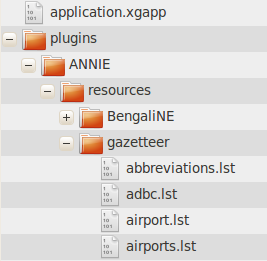
\includegraphics[width=0.3\textwidth]{app-zip-structure.png}
\end{center}
\caption{Application ZIP structure}
\label{fig:cloudappzipstructure}
\end{figure}

The easiest way to build such a package is simply to save your application in
GATE Developer using the "Export for GATE Cloud" option, which produces a ZIP
file containing an {\tt application.xgapp} and all its required resources in one
click.

%%%%%%%%%%%%%%%%%%%%%%%%%%%%%%%%%%%%%%%%%%%%%%%%%%%%%%%%%%%%%%%%%%%%%%%%%%%%%
\subsection{The GATE Cloud environment}
%%%%%%%%%%%%%%%%%%%%%%%%%%%%%%%%%%%%%%%%%%%%%%%%%%%%%%%%%%%%%%%%%%%%%%%%%%%%%%

For many GATE applications that just use the standard pure-Java ANNIE
components, the basic information above is all you need to know to run your
application on GATE Cloud.  But for more advanced applications that involve
custom PRs, platform-specific native helpers (such as an external tagger), or
other components that need to know the path where they are installed, you will
need to know a little more about the environment in which your application will
be running.

\subsubsection{Hardware and software}

GATE Cloud annotation jobs are executed on virtual 64-bit (x86\_64) GNU/Linux
servers in the cloud, specifically Ubuntu 14.04 LTS (Trusty Tahr).  The GATE
application is run using the open-source GCP tool\footnote{Source code is
  available in the subversion repository at\\
  {\tt http://svn.code.sf.net/p/gate/code/gcp/trunk}} on Oracle Java 8
(currently 1.8.0\_71).  The current offering uses the Amazon EC2 cloud, and runs
jobs on their 'm3.xlarge' machines which provide 4 virtual CPU cores and 15GB of
memory, of which 13GB is available to the GCP process.

The jobs are run using GATE Embedded version 8.3, and your application must use
GATE plugins that are compatible with this version. The following plugins are
pre-loaded by default in order to support additional input data formats:
\verb!Format_Twitter!, \verb!Format_MediaWiki!, \verb!Format_PubMed!,
\verb!Format_FastInfoset! and \verb!Format_DataSift!.

The GCP (GATE Cloud Paralleliser) process is configured for 'headless' operation
(\verb^-Djava.awt.headless=true^), and your code should not assume that a GUI
display is available.

GCP loads one copy of your \verb!application.xgapp! in the
\javadoclink{gate/util/persistence/\-PersistenceManager.html\#loadObjectFromFile\-\%28java.io.File\%29}{usual way}
using the PersistenceManager.  It then uses the GATE
\javadoclink{gate/Factory.html\#duplicate\-\%28gate.Resource\%29}
{duplication mechanism}
to make a further 5 independent copies of the loaded application, and runs 6
parallel threads to process your documents.  For most PRs this duplication
process is essentially equivalent to loading the original \verb^application.xgapp^ 6
times but if you are writing a custom PR you may wish to consider implementing
a custom duplication strategy.

\subsubsection{Directories}

The application ZIP file will always be unpacked in a directory named
\begin{small}\verb^/gatecloud/application^\end{small} on the cloud server.  
Thus the application file will
always be\\
\verb^/gatecloud/application/application.xgapp^ and if any of your
components need to know the absolute path to their resource files you can work
this out by prepending \verb^/gatecloud/application/^ to the path of the entry
inside your ZIP package.  The user account that runs the GCP process has full
read and write access in the \verb^/gatecloud/application^ directory, so if any of
your components need to create temporary files then this is a good place to put
them.  Any files created under \verb^/gatecloud/application^ will be lost when the
current batch of documents has been processed.

The directory \verb^/gatecloud/batch/output^ is where GCP will write any output
files specified by the output definitions you supply when running an annotation
job.  All files created under this directory will be packaged up into ZIP files
when the batch of documents has been processed and made available for download
when the job has completed.  Thus, any additional output files that your
application creates and that need to be returned to the user should be placed
under \verb^/gatecloud/batch/output^.

Your code should not assume it has permission to read and write any files
outside these two locations.

\subsubsection{Native code components}

Many PRs are simply wrappers around non-Java tools, for example third-party
taggers of various kinds.  If your application requires the use of any non-Java
components you must ensure that the version you include in your ZIP package is
the one that will run on Linux x86\_64, and in particular on Ubuntu 10.10.  The
cloud processing servers have
\htlink{http://uec-images.ubuntu.com/server/\-releases/\-maverick/\-release-20101225/\-ubuntu-10.10-server-uec-amd64.manifest}{a reasonable set of packages}
installed by default, including a basic install of Perl and Python, sed, awk
and bash.  To request additional packages please 
\htlink{https://cloud.gate.ac.uk/info/contact/}{contact GATE Cloud support} with
your requirements.  If you want to be sure your code will work on GATE Cloud
then the best approach is to sign up for your own account at
\htlink{http://aws.amazon.com}{Amazon Web Services}, run your own instance of the
\htlink{http://uec-images.ubuntu.com/server/releases/maverick/release-20101225/}
{same machine image} that GATE Cloud uses and test the software yourself.  
As Amazon charges by the hour with no up-front fees this should cost you very 
little.

As your code will be running in a Linux environment, remember that any native
executable or script that your application needs to call must be marked with
execute permission on the filesystem.  GATE Cloud uses the standard Info-ZIP
"unzip" tool to unpack the application ZIP package, which respects permission
settings specified in the ZIP file, so if you build your package using the
corresponding "zip" tool the permissions will be preserved.  However, many ZIP
file creation tools (including GATE's "Export for GATE Cloud") do not preserve
permissions in this way.  Therefore GATE Cloud also supports an alternative
mechanism to mark files as executable.

Once the application ZIP has been unpacked, we look through the resulting
directory tree for files named \verb^.executables^.  If any such file is found,
we treat each line in the file as a relative path, and set the execute flag on
the corresponding file in the file system.  For example, imagine the following
structure:

\begin{small}
\begin{verbatim}
application.xgapp
plugins
  - MyTagger
    - resources
      - tagger.sh
      - postprocessor.pl
\end{verbatim}
\end{small}

Here, tagger.sh and postprocessor.pl are scripts that need to be marked as
executable, so we could create a file \verb^plugins/MyTagger/.executables^
containing the two lines:

\begin{small}
\begin{verbatim}
resources/tagger.sh
resources/postprocessor.pl
\end{verbatim}
\end{small}

or equivalently, create \verb^plugins/MyTagger/resources/.executables^ containing

\begin{small}
\begin{verbatim}
tagger.sh
postprocessor.pl
\end{verbatim}
\end{small}

Either way, the effect would be to make the GATE Cloud processing machine
mark the relevant files as executable before running your application.

\subsubsection{Security and privacy}

GATE Cloud does not run a separate machine for each annotation job.  Instead
it splits each annotation job up into manageable pieces (referred to as tasks),
puts these tasks into a queue, and runs a collection of processing machines
(referred to as "nodes") that simply take the next task from the queue whenever
they have finished processing their previous task.  While a task is running it
has exclusive use of that particular node - we never run more than one task on
the same node at the same time - but once the task is complete the same node
will then run another task (which may or may not be part of the same annotation
job).

To ensure the security and privacy of your code and data, the node takes the
following precautions:

\begin{itemize}
\item All GCP processes are run as an unprivileged user account which only has
  write permission in a restricted area of the filesystem (see above).
\item At the end of every task, {\bf all} processes running under that user ID are
  forcibly terminated (so there's no risk of a stray or malicious background
  process started by a previous task being able to read your data).
\item The \verb^/gatecloud/application^ and \verb^/gatecloud/batch^ directories are
  completely deleted at the end of every task (whether the task completed
  successfully or failed) so your data will not be left for the following task
  to see.
\end{itemize}

\else % ifprintedbook

\subsect[sec:cloud:details]{Where to find more details}

Detailed documentation on the GATE Cloud platform can be found at
\htlinkplain{https://cloud.gate.ac.uk/info/help}, including

\begin{itemize}
\item Documentation for the various REST APIs
\item Details of how to prepare your own custom pipeline to run as a batch job
\end{itemize}

A Java client library and command-line tool for the REST APIs can be found at
\htlinkplain{https://github.com/GateNLP/cloud-client}, with extensive
documentation on its own GitHub wiki, along with example code showing how you
can call the APIs from other programming languages.

Finally, you can use the \htlink{https://gate.ac.uk/mail/}{GATE-users mailing
list} if you have any questions not covered by the documentation.

\fi % end of ifprintedbook/else
